\section{Istruzioni per l'utilizzo}
\subsection{Requisiti}
Di seguito vengo riportati i requisiti minimi per garantire il funzionamento del prodotto Colletta:
\subsubsection{Requisiti software}
\begin{itemize}
\item {Sistema operativo:} qualsiasi;
\item {Browser web:} ogni browser web aggiornato all'ultima versione, tranne Internet Explorer e Edge.
\end{itemize}
Si specifica inoltre che JavaScript deve essere abilitato sul browser per il corretto funzionamento dell’applicazione.
\subsubsection{Requisiti hardware}
Connessione ad Internet.
\subsection{Componenti principali}
Questa sezione serve per definire i termini con cui chiamare gli elementi che compongono la pagina dell'applicazione.
Componenti principali:
\begin{itemize}
    \item Barra del menu;
    \item {Sidebar}\ped{G};
    \item Contenuto della pagina;
    \item footer.
\end{itemize}

\begin{figure}[H]
    \centering
    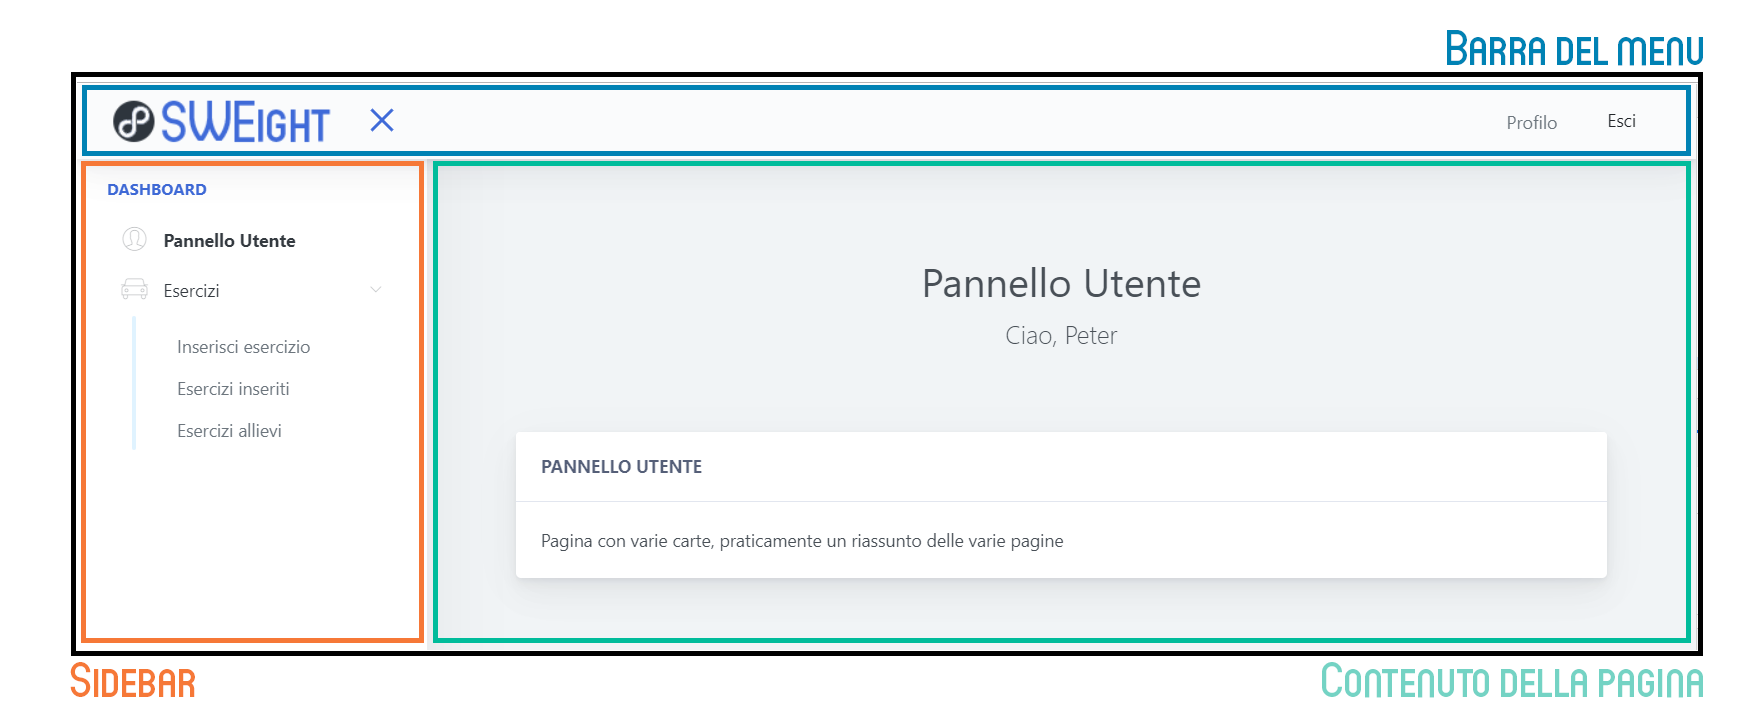
\includegraphics[width=17cm]{sez/img/istruzioni/dashboardMod.png} 
    \caption{Definizione componenti}\label{fig:1}
\end{figure}

\begin{figure}[H]
	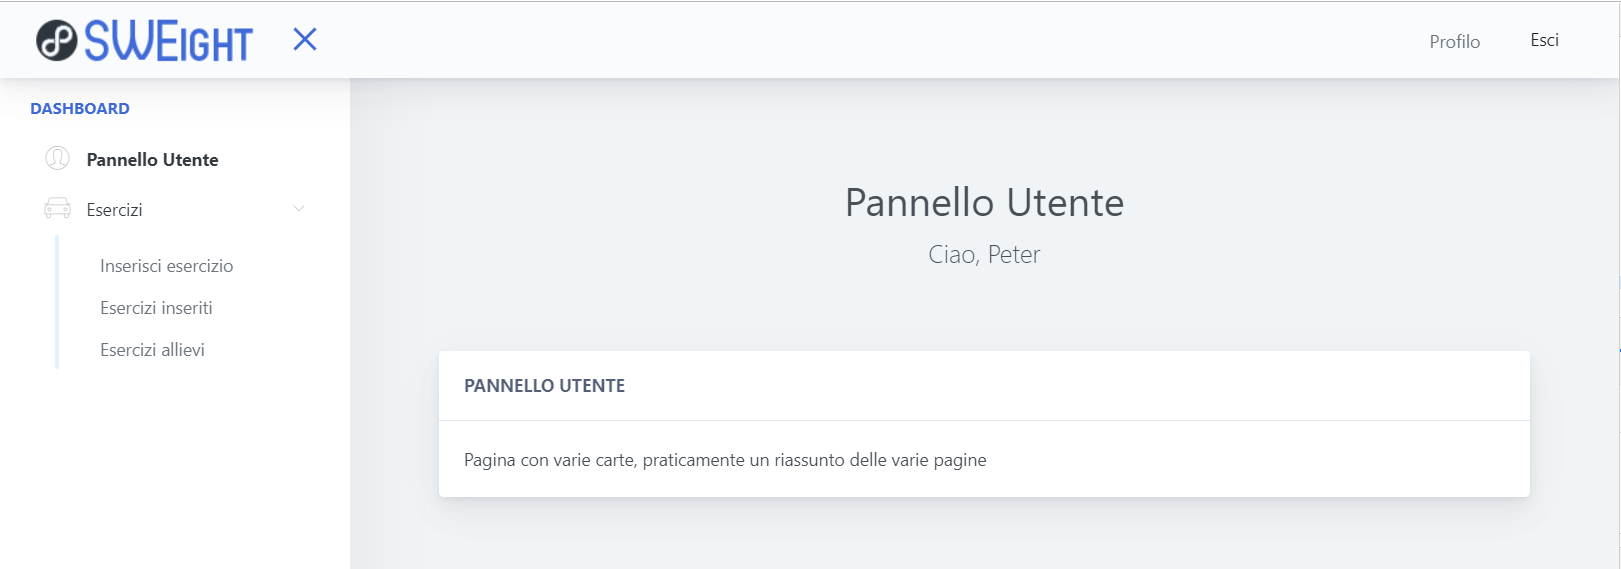
\includegraphics[width=1\linewidth]{sez/img/istruzioni/dashboard.PNG}
	\caption{Indice di Gulpease nel periodo di Progettazione}
\end{figure}

\subsection{Autenticazione}
\subsubsection{Registrazione}
Senza una registrazione non è possibile accedere alla piattaforma.
\subsubsection{Login}
Dopo aver effettuato la registrazione si accede tramite email e password.
\subsubsection{Logout}
Per effettuae il {logout}\ped{G} si deve cliccare su la voce \textit{Esci} dal menu principale